\newpage
\changeindent{0cm}
\section{要素技術}
\changeindent{2cm}

本章では,実験に関連する要素技術について説明する.

\changeindent{0cm}
\subsection{半教師あり学習}
\changeindent{2cm}
半教師あり学習 (Semi Supervised Learning: SSL)\cite{zhu2005semi,chapelle2009semi} は
大量のラベルなしデータと少量のラベル付きデータを用いて学習を行う手法である.


\changeindent{0cm}
\subsection{疑似ラベル}
\changeindent{2cm}
疑似ラベル (Pseudo Label)\cite{lee2013pseudo} はあるモデルによって予測されるラベルなしデータに対する暫定的なラベルである.
 SSL では疑似ラベルを付与したデータをラベル付きデータに混ぜて学習することで各ラベル同士に対する確率分布を粗密なものにする作用があり,正則化\cite{grandvalet2006entropy}の役割をする.データ数を $N$\ ,あるモデルによる予測確率を $q_b$\ ,予測確率 $p, q$\ に対する Cross Entropy Loss を ${\rm H}(p,q)$\ ,閾値を $\tau$ とするとき,(\ref{quadPL})式で与えられる.
 
 \begin{equation}
 \hat{q}_b = {\rm argmax}(q_b)
 \end{equation}
 \begin{equation}
 \label{quadPL}
 \frac{1}{N}\sum^{N}_{b=1}
 {\mathbb{1}({\rm max}(q_b)\geq\tau){\rm H}(\hat{q}_b,q_b)}
 \end{equation}
 
\changeindent{0cm}
\subsection{FixMatch}
\changeindent{2cm}
FixMatch\cite{sohn2020fixmatch}\ は\ SSL\ の一つである.
図\ref{fig:FixMatch}に\ FixMatch\ の概略図を示す.
疑似ラベルと Consistency Regularization の二つの正則化手法を
統合させた手法である.


\begin{figure}[h]
	\begin{center}
		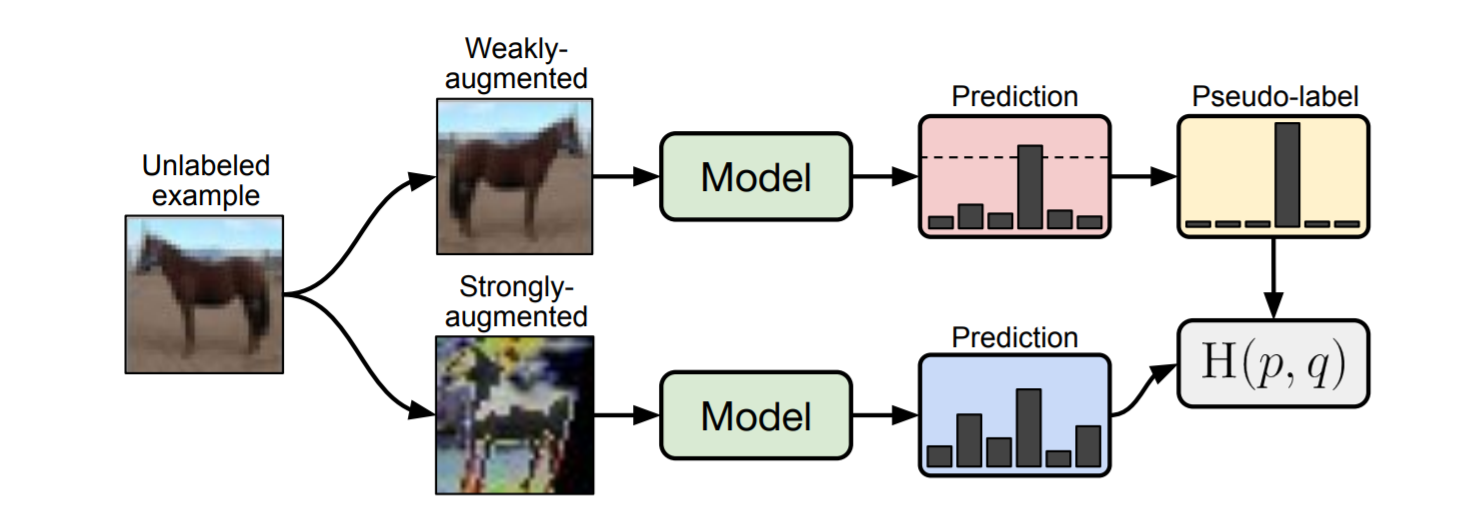
\includegraphics[scale=0.6]{./images/FixMatch.PNG}
		\caption[FixMatch の概略図]
		{FixMatch の概略図 (: 文献\cite{sohn2020fixmatch}の Figure 1 を参照\label{fig:FixMatch})}
	\end{center}
\end{figure}

\changeindent{0cm}
\subsubsection{RandAugment}
\changeindent{2cm}
RandAugment \cite{cubuk2020randaugment} とは,データ拡張手法の一つであり,
チューニングするパラメータは $N$ と $M$ の二種類で,複数あるデータ変換操作のうちランダムに $N$ 個選択し
変換強度 $M$ で順に適用する手法である.FixMatch では強変換として用いられる.


\changeindent{0cm}
\subsubsection{Consistency Regularization}
\changeindent{2cm}
Consistency Regularization \cite{zhang2019consistency} は正則化手法の一つであり,
画像による変換の前後で予測値が変わらないようなロスを与える.ラベルなしデータを$u_b$\ ,
 $\alpha(\cdot)$ を画像変換,$p_{\rm m}(y|x)$ を入力 $x$ に対するモデルの出力とすると,
(\ref{quadCR})式で与えられる.

\begin{equation}
\label{quadCR}
\sum^{N}_{b=1}{||p_{\rm m}(y|\alpha_1(u_b)) - p_{\rm m}(y|\alpha_2(u_b))||^2_2}
\end{equation}

\changeindent{0cm}
\subsubsection{更新}
\changeindent{2cm}
まず,バッチサイズを $B$ としラベル付きデータを ${\cal X} = {(x_b, p_b): b \in (1, ... ,B)}$ 
としたとき,ラベル付きデータに対するロスを ${\ell}_{\rm s}$ とすると,(\ref{quadLs})式で与えられる.

\begin{equation}
\label{quadLs}
{\ell}_{\rm s} = \frac{1}{B}\sum^{B}_{b=1}{\rm H}(p_b,p_{\rm m}(y|\alpha(x_b)))
\end{equation}

また,ラベルなしデータに対するロス ${\ell}_{\rm u}$ は,(\ref{quadPL}),(\ref{quadCR})式より,

\begin{equation}
\label{quadLu}
{\ell}_{\rm u} = \frac{1}{\mu B}\sum^{\mu B}_{b=1}
{\mathbb{1}({\rm max}(q_b)\geq\tau){\rm H}(\hat{q}_b,p_{\rm m}(y|{\cal A}(u_b)))}
\end{equation}

となる.このとき,$\mu$ はバッチ内のラベル付きデータに対するラベルなしデータの比率,$\cal A(\cdot)$は強変換である.

従って,ラベルなしデータの重みを$\lambda$	として,バッチ全体のロスは ${\ell}_{\rm s}+\lambda {\ell}_{\rm u}$ となる.

\changeindent{0cm}
\subsection{SimCLR}
\changeindent{2cm}
Simple framework for Contrastive Learning of visual Representation(SimCLR)\cite{chen2020simple}は SSL の一つである.
図\ref{fig:SimCLR}に概略図を示す.モデルの構造は Encoder,Projection Head,Classsifier
から構成されており, Encoder と Projection Head に対して,全データを用いて Contrastive Learning によって学習する.次に学習済みの Encoder と Classifier に対して,ラベル付きデータを用いて Classifier の学習を行う.最後にモデルの蒸留\cite{hinton2015distilling}を行うことで最終的なモデルを得る.

\begin{figure}[h]
	\begin{center}
		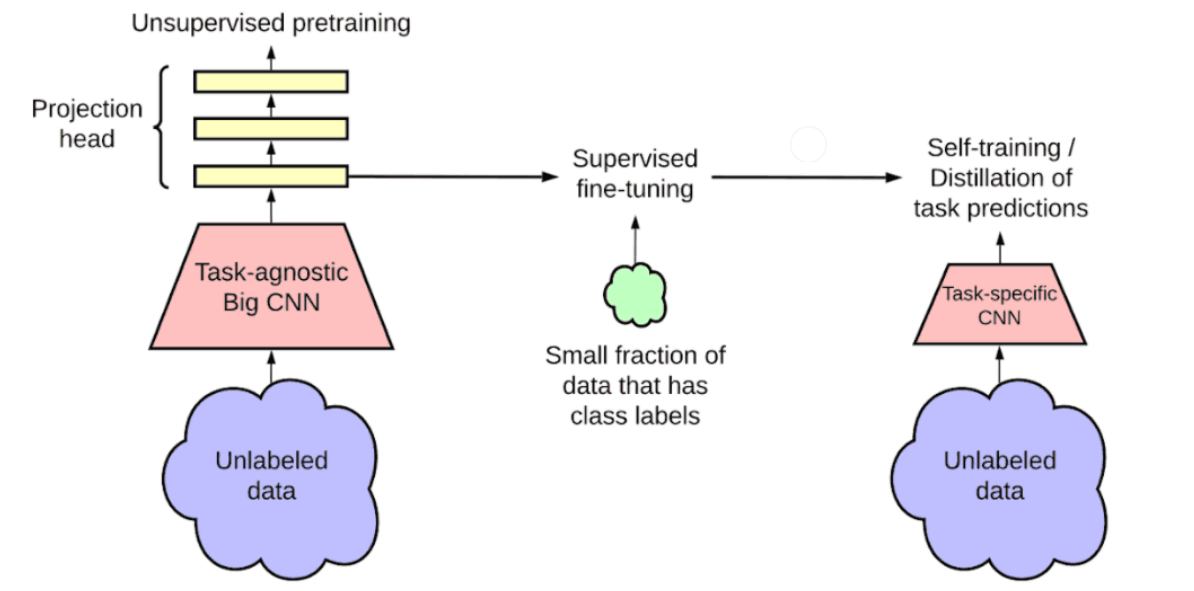
\includegraphics[scale=1.0]{./images/SimCLR.png}
		\caption[SimCLR の概略図]
		{SimCLR の概略図 (: 文献\cite{chen2020big}の Figure 3 を参照\label{fig:SimCLR})}
	\end{center}
\end{figure}

\changeindent{0cm}
\subsubsection{Cotrastive Learning}
\changeindent{2cm}
Contrastive Learning (CL)\cite{tian2020makes} とは特徴表現を獲得するための
自己教師あり学習\cite{doersch2017multi}のひとつである.
ある画像変換をした画像のペアについて元画像が一致するか否かを識別するタスクであり,
一つの画像から得られる特徴表現が画像変換によって
画像の持つ意味が大きく変化しないような Encoder を獲得することができる.
具体的な方法について,バッチ内の画像枚数を $N$ 枚とすると, Data Augmentation によって2倍に増やしたとき,
各画像に対して正例は1枚,負例は $2(N-1)$ 枚となる.このとき特徴ベクトル間の距離として cos 類似度を用いると,(\ref{sim})式で表される.また,正例との距離を小さくかつ,負例との距離を大きくするために正例のペア $({\bm z}_i,{\bm z}_j)$ に対するロス $\ell(i, j)$ は(\ref{quad_posl})式で表され,
バッチ全体のロス$\mathcal L$は(\ref{quad_L})式で表される.

\begin{equation}
\label{sim}
{\rm sim}({\bm u},{\bm v}) = {\bm u}^{\rm T}{\bm v}/\|{\bm u}\|\|{\bm v}\|
\end{equation}

\begin{equation}
\label{quad_posl}
\ell(i, j) = - {\rm log}\frac{{\rm exp}({\rm sim}({\bm z}_i, {\bm z}_j)/ \tau)}
{\sum_{k=1}^{2N}\mathbb{1}_{[k \neq i]}{\rm exp}({\rm sim}({\bm z}_i, {\bm z}_k)/ \tau)}
\end{equation}

\begin{equation}
\label{quad_L}
\mathcal L = \frac{1}{2N}\sum_{k=1}^{N}[\ell(2k-1,2k)+\ell(2k,2k-1)]
\end{equation}


\changeindent{0cm}
\subsection{ResNet}
\changeindent{2cm}
Residual Network (: ResNet)\cite{he2016deep} は Deep Neural Network (: DNN)\cite{larochelle2009exploring} のモデルの一つであり,
 DNNにおいて層を深くすることで発生する劣化問題及び勾配消失問題\cite{hochreiter1998vanishing}を解消するために残差についての学習を行うモデルである.図\ref{fig:ResBlock}に ResNet の構成要素である Residual Block の構造を示す.
2層の畳み込み層とショートカットを足し合わせた構造となっている.

\begin{figure}[h]
	\begin{center}
		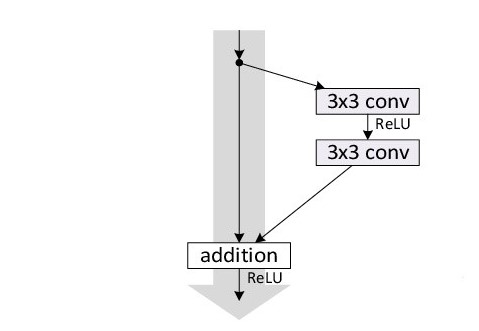
\includegraphics[scale=0.5]{./images/ResBlock.jpg}
		\caption[Residual Block の構造]
		{Residual Block の構造 (: 文献\cite{he2016identity}の Figure 2.(a) を参照\label{fig:ResBlock})}
	\end{center}
\end{figure}

\changeindent{0cm}
\subsection{Genetic Algorithm}
\changeindent{2cm}
遺伝的アルゴリズム (Genetic Algorithm: GA)\cite{whitley1994genetic} とは,生物の進化を模倣した組合せ最適化問題のアルゴリズムである.解の要素の最小単位を遺伝子,遺伝子の集まりである解を個体として表現する.また個体の集合を世代とし,各個体の計算された適応度をもとに選択,交叉,突然変異の3つの操作によって新たな個体群を生成し,次世代の個体集合とする.繰り返し世代を重ねることで最適解を探索する.
個体の基本的なエンコーディング方法として,バイナリ型,順列型,実数型,整数型がある.
本研究では整数型について扱うため,以下整数型を前提とした説明をする.

\changeindent{0cm}
\subsubsection{選択}
\changeindent{2cm}
選択\cite{blickle1996comparison}は自然淘汰をもとにした操作であり,個体の適応度にもとづき次世代に残される個体を選ぶものである.
以下のものがあげられる.
\begin{itemize}
	\setlength{\leftskip}{4.5cm}
	\item[エリート選択\cite{murata1996multi} : ]世代における適応度の最も高い個体を他の操作を行わず次世代に残す手法である.
	\item[トーナメント選択 : ]個体群からランダムに決められた数(: トーナメントサイズ)取り出し,
	その中で適応度の最も高い個体を選択する手法である.
\end{itemize}

\changeindent{0cm}
\subsubsection{交叉}
\changeindent{2cm}
交叉は生物の交配をもとにした操作であり,2つの個体から新たな2つの個体を生成するものである.
以下のものがあげられる.
\begin{itemize}
	\setlength{\leftskip}{3cm}
	\item[二点交叉 : ]対象となる2つの個体を同じ遺伝子座で3つに分割を行い,いずれかを入れ替える手法である.
	\item[一様交叉 : ]対象となる2つの個体についてある遺伝子座ごとにある確率で入れ替えを行う手法である.
\end{itemize}

\changeindent{0cm}
\subsubsection{突然変異}
\changeindent{2cm}
個体の遺伝子を変化させる操作で,局所探索になることを防ぐ.
乱数によって他の取りうる値に変化させる.また,突然変異率を上げすぎるとランダム探索となり,
収束しなくなるため,高くても数\%に設定されることが多い.


%CIFAR10\cite{krizhevsky2009learning}

%CL\cite{khosla2020supervised}